\section{Societal Impact of COVID-19}

So far, COVID-19 has had an enormous impact on societies both local and global. There has been a harsh decline in the number of people visiting the hospital, even in urgent situations. For instance, a study regarding paediatric urgency care in Italy showed a decline in visits of 84 percent from 2019 to 2020. This therefore has a long-term negative impact on paediatric health \citep{manzoni_impact_nodate}.

\begin{figure}[H]
    \centering
    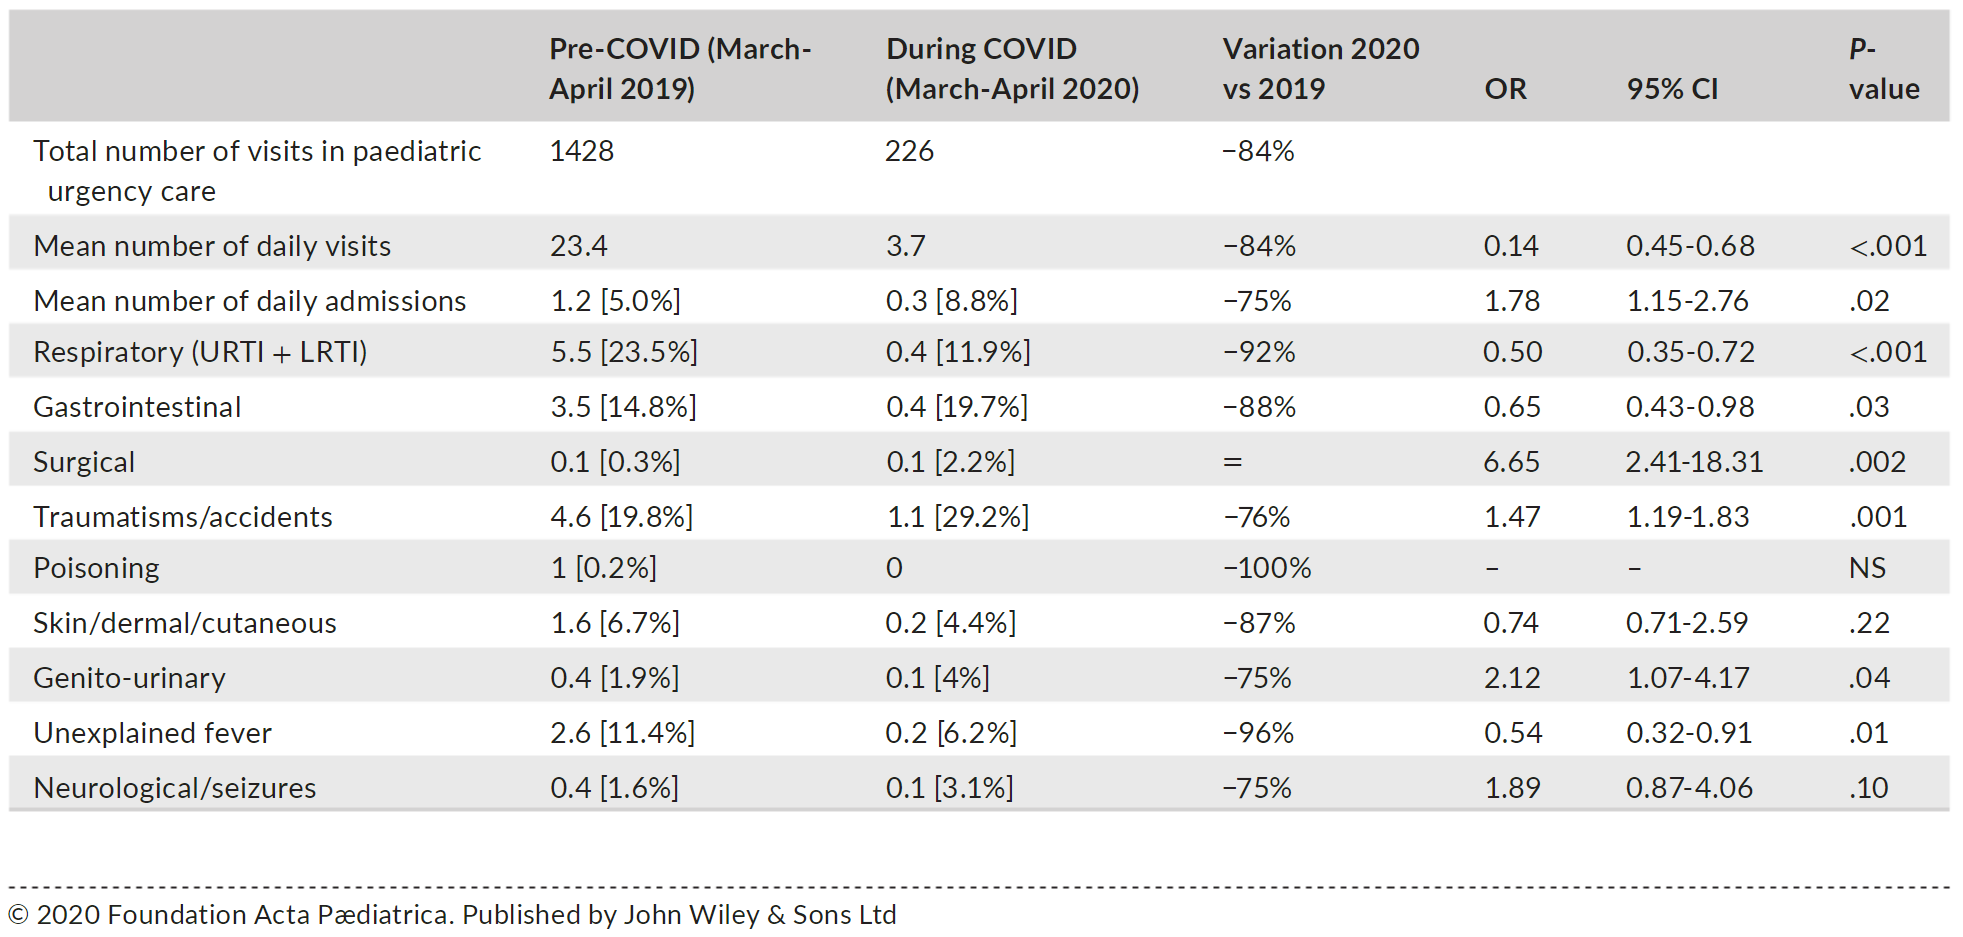
\includegraphics[width=\textwidth]{0_billeder/Covid impact hospitals.PNG}
    \caption{This table shows the visits to paediatric urgency care in 2019 compared to during COVID-19 \citep{manzoni_impact_nodate}}
    \label{fig:Covid-Hospital}
\end{figure}

Similarly, the COVID-19 pandemic has caused a tremendous surge in volatility in the stock market. Volatility is the liability of the stock market to change rapidly. This is the third highest peak since 1900, as seen in figure \ref{fig:Covid-Economy} only outdone by the great crash of Wall Street in 1929 and Black Monday in 1987 \citep{baker_unprecedented_2020}.

\begin{figure}[H]
    \centering
    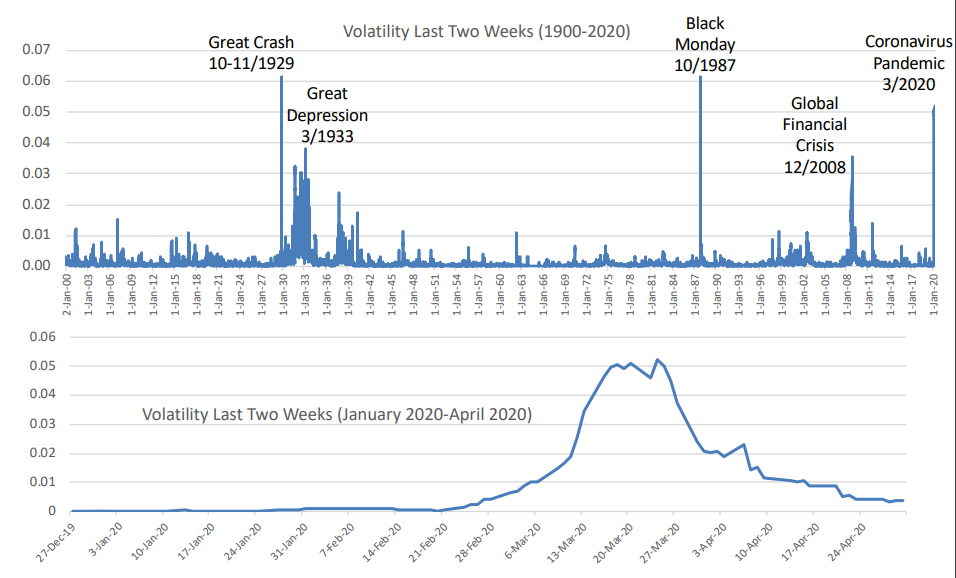
\includegraphics[width=\textwidth]{0_billeder/Covid impact Economy.PNG}
    \caption{This graph shows the spikes of volatility in the stock-market since 1900 \citep{baker_unprecedented_2020}}
    \label{fig:Covid-Economy}
\end{figure}

When dealing with a pandemic like COVID-19, it is important to consider not only the effect on mental health that may be caused by the existence of the virus alone but also the effect that preventative measures can have on mental health.

COVID-19 spreads rapidly with human-to-human contact, which in turn has caused a surge in anxiety, stress, xenophobia and the like. The consequences of these increases in mental strain on the general population has also led to behaviours like hoarding, mistrust in authority and similar that negatively affect the prevention and mitigation of COVID-19 \citep{javed_coronavirus_2020}.